\documentclass[border=4pt]{standalone}
\usepackage{amsmath,amssymb}
\usepackage{tikz}
\usetikzlibrary{arrows.meta,calc}
\begin{document}
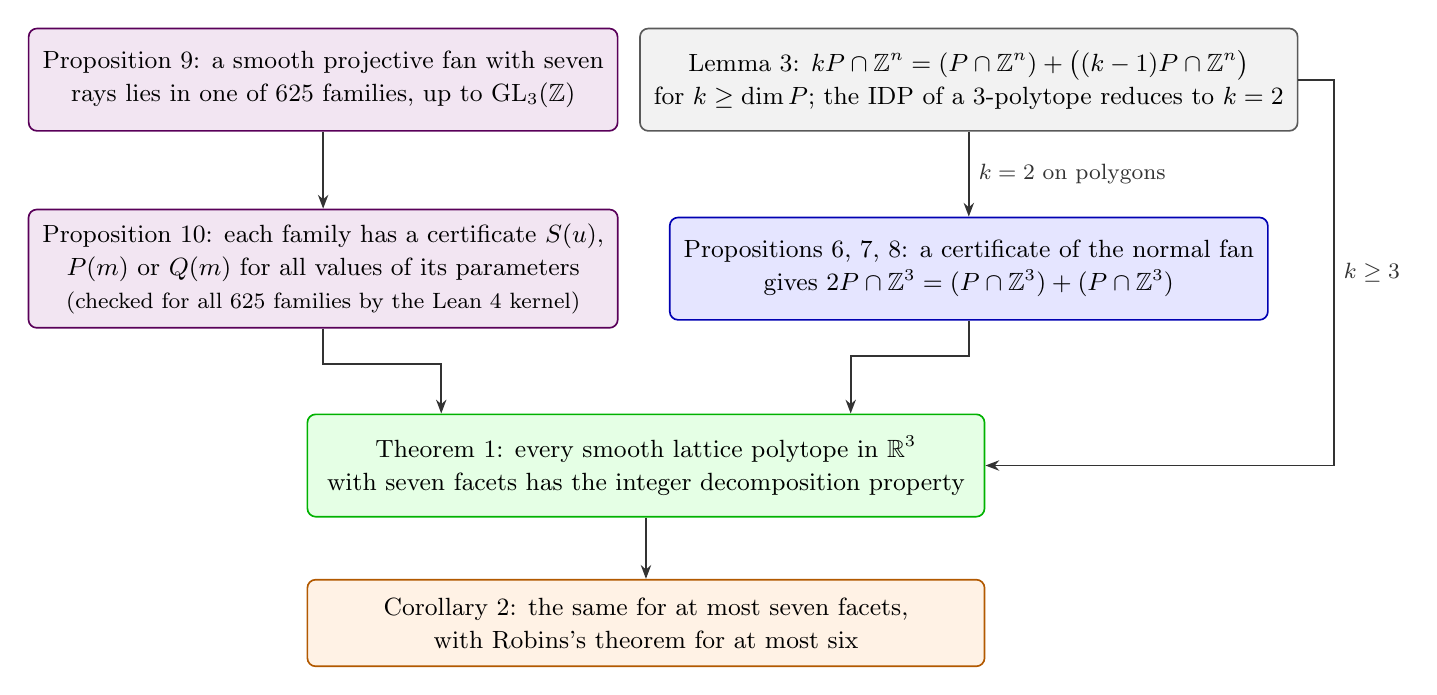
\begin{tikzpicture}[
  box/.style={draw=#1!70!black,fill=#1!10,rounded corners=3pt,line width=0.6pt,
              align=center,font=\small,inner sep=5pt,minimum height=13mm,minimum width=7.2cm},
  box/.default=gray,
  arr/.style={-{Stealth[length=5pt]},line width=0.6pt,gray!40!black}]
  \node[box=violet] (cls) at (-4.1,0)
    {Proposition 9: a smooth projective fan with seven\\[1pt]
     rays lies in one of $625$ families, up to $\mathrm{GL}_3(\mathbb{Z})$};
  \node[box=gray] (red) at (4.1,0)
    {Lemma 3: $kP\cap\mathbb{Z}^n=(P\cap\mathbb{Z}^n)+\bigl((k-1)P\cap\mathbb{Z}^n\bigr)$\\[1pt]
     for $k\ge\dim P$; the IDP of a $3$-polytope reduces to $k=2$};
  \node[box=violet] (cert) at (-4.1,-2.4)
    {Proposition 10: each family has a certificate $S(u)$,\\[1pt]
     $P(m)$ or $Q(m)$ for all values of its parameters\\[1pt]
     {\footnotesize (checked for all $625$ families by the Lean~4 kernel)}};
  \node[box=blue] (crit) at (4.1,-2.4)
    {Propositions 6, 7, 8: a certificate of the normal fan\\[1pt]
     gives $2P\cap\mathbb{Z}^3=(P\cap\mathbb{Z}^3)+(P\cap\mathbb{Z}^3)$};
  \node[box=green,minimum width=8.6cm] (thm) at (0,-4.9)
    {Theorem 1: every smooth lattice polytope in $\mathbb{R}^3$\\[1pt]
     with seven facets has the integer decomposition property};
  \node[box=orange,minimum width=8.6cm,minimum height=11mm] (cor) at (0,-6.9)
    {Corollary 2: the same for at most seven facets,\\[1pt]
     with Robins's theorem for at most six};
  \draw[arr] (cls) -- (cert);
  \draw[arr] (red) -- node[right,font=\footnotesize]{$k=2$ on polygons} (crit);
  \draw[arr] (cert.south) -- ++(0,-0.45) -| ([xshift=-2.6cm]thm.north);
  \draw[arr] (crit.south) -- ++(0,-0.45) -| ([xshift=2.6cm]thm.north);
  \draw[arr] (red.east) -- ++(0.45,0) |- node[pos=0.25,right,font=\footnotesize]{$k\ge3$} (thm.east);
  \draw[arr] (thm) -- (cor);
\end{tikzpicture}
\end{document}
